\documentclass{beamer}
\usetheme{Madrid}

\title[Оценивание значимости выравнивания]{Задачи оценивания значимости выравнивания при помощи скрытых марковских моделей}
\author[Власенко Даниил]{Власенко Даниил Владимирович \\ Научный руководитель: к.ф.-м.н. Коробейников А.И.}
\date[Декабрь 2021]{Санкт-Петербург\\Декабрь 2021}
\institute[]{Санкт-Петербургский государственный университет\\ Кафедра "Статистического моделирования"} 

\usepackage{amsmath,amssymb,amsthm,amscd,amsfonts}
\usepackage[utf8]{inputenc}
\usepackage[russian]{babel}
\usepackage{wrapfig}

\newtheorem{defenition}{Определение}

\begin{document}
	\begin{frame}
		\titlepage
	\end{frame}

	\begin{frame}{Выравнивание последовательностей}
		\begin{defenition}
			Выравнивание последовательностей  "--- размещение двух или более последовательностей друг под другом таким образом, чтобы было легче увидеть их схожие участки.
		\end{defenition}
	
		\begin{center}
			\begin{tabular}{cccccccc}
				A&C&E&A&A&F&A&E\\
				C&E&A&F&D&C&E&\\
			\end{tabular}
		\end{center}
		\begin{center}
			\begin{tabular}{ccccccccc}
				A&C&E&A&A&F&A&—&E\\
				—&C&E&A&—&F&D&C&E\\
			\end{tabular}
		\end{center}
	
		\begin{defenition}
			Значимость выравнивания "--- действительное число $s$, отражающее сходство последовательностей.
		\end{defenition}
	\end{frame}

	\begin{frame}{Ложноположительная вероятность}
		\begin{itemize}
			\item достаточно ли высокая значимость, чтобы считать последовательность не шумом, или шум мог добиться такой значимости.
			\item достаточно ли низкая значимость, чтобы считать последовательность шумом, или не шум мог получить такую значимость. 
		\end{itemize}
	
		\begin{defenition}
			Ложноположительная вероятность значимости $s$ "--- это вероятность того, что шум получит значимость равную или выше $s$. 
		\end{defenition}
	\end{frame}

	\begin{frame}{Модели}
		\begin{defenition}
			Пусть $X_{n}$ и $Y_{n}$ дискретные стохастические процессы, $n \geq 1$. Пара $(X_{n}, Y_{n})$ называется скрытой марковской моделью, если
			\begin{itemize}
				\item $X_{n}$~--- марковский процесс, поведение которого напрямую не наблюдается ("скрытый");
				\item $P(Y_{n} = y_{n}|X_{1} = x_{1},\dots, X_{n} = x_{n}) = P(Y_{n}|X_{n}=x_{n})$ для любого $n \geq 1$, где $x_{1},\dots,x_{n}$~--- значения, принимаемые процессом  $X_{n}$ (\textbf{состояния модели}), $ y_{n}$~--- значение, принимаемое процессом $Y_{n}$ (\textbf{наблюдаемый символ модели}).
			\end{itemize}
		\end{defenition}		
	\end{frame}

	\begin{frame}{Модели}
		\begin{figure}[h]
			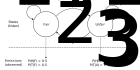
\includegraphics[width=10cm]{../report/figure1}
		\end{figure}
	\end{frame}

	\begin{frame}{Модели}
		\begin{figure}[h]
			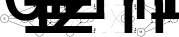
\includegraphics[width=12cm]{../report/figure2}
		\end{figure}		
	\end{frame}

	\begin{frame}{Модели}
		\begin{defenition}
			\textit{Вероятность последовательности} $D$ может интерпретироваться и считаться по-разному "--- алгоритмом \textit{Витерби} или \textit{Форвард} алгоритмом.
		\end{defenition}
		
		\begin{equation}
			s_{max}(D) = \underset{\pi \in \pi_{D}}{max}(s(\pi)),
		\end{equation}
	
		\begin{equation}
			s_{fw}(D) = \sum_{\pi \in \pi_{D}}s(\pi).
		\end{equation}
	
		\begin{equation}
			Z(D, T)	= \sum_{\pi \in \pi_{D}}s(\pi)^{\frac{1}{T}}.
		\end{equation}
	\end{frame}	

	\begin{frame}{Модели}
		Мы предполагаем наличие простой фоновой модели $B$ для последовательностей длины $L$ такой, что все $L$ символьных позиций независимы и одинаково распределены в соответствии с некоторым распределением $Pr(d|B)$, где $d$ отражает возможный наблюдаемый символ:
		\begin{equation}
			Pr(D|B) = \prod_{i=1}^{L}Pr(d_{i}|B),
		\end{equation}
		где $d_{i}$ "--- это $i$-ый наблюдаемый символ последовательности $D$.
	\end{frame}

	\begin{frame}{Постановка математической задачи}
		\begin{defenition}
			Ложноположительная вероятность значимости $s_{0}$ для строк длины $L$:	
			\begin{equation}
				fpr(s_{0}) =  \sum_{D \in D_{L}} Pr(D|B) \Theta(s(D) \geq s_{0}),
			\end{equation}
			где $Pr(D|B)$ "--- условная вероятность последовательности $D$, описываемая фоновой моделью, $s(D)$ "--- вероятность последовательности $D$, считаемая профильной СММ, и
			\[
			\Theta(s(D) \geq s_{0}) = 
			\begin{cases}
				1, & s(D) \geq s_{0}\\
				0, & s(D) < s_{0}
			\end{cases}.
			\]
		\end{defenition}		
	\end{frame}
	
	\begin{frame}{Алгоритм}
		Вычисление $fpr(s_{0})$ через формулу 5 обычно неосуществимо, значение $fpr(s_{0})$ может быть оценено через выборку по значимости. 
		
		\vspace{0.5cm}
		
		Пусть $P(D|T)$ "--- это условная вероятность строки $D$ относительно некоторой модели строк длины $L$ параметризованной значением $T$. Тогда можно переписать $fpr(s_{0})$:		
		
		\begin{equation}
			fpr(s_{0}) = \sum_{D \in D_{L}} Pr(D|T) f(D,s_{0}),
		\end{equation}
		где
		\begin{equation}
			f(D,s_{0}) = \frac{Pr(D|B) \Theta(s(D) \geq s_{0})}{Pr(D|T)}.
		\end{equation}				
	\end{frame}

	\begin{frame}{Алгоритм}
		Определим модель, используемую для выборки по важности параметризованную $T$:		
		
		\begin{equation}
			Pr(D|T) = \frac{P(D|B)Z(D,T)}{Z(T)},
		\end{equation}							
		где 
		\begin{equation}
			Z(T) = \sum_{D \in D_{L}}Pr(D|B)Z(D,T).
		\end{equation}
		Подставив определение $Pr(D,T)$ в уравнение 7 получим
		\begin{equation}
			f(D,s_{0}) = \frac{Z(T)\Theta(s(D) \geq s_{0})}{Z(D,T)}.
		\end{equation}	
	\end{frame}

	\begin{frame}{Результаты}
		Вычислим оценку $\widehat{fpr}(s_{0})$ для строк длины $L=100$, состоящих из 5 символов, и доверительные интервалы уровня $\gamma = 0.99$:
		\begin{center}
			\begin{tabular}{cccc}
				$s_{0}$&T&$\widehat{fpr}(s_{0})$&$[c_{1}(\gamma);c_{2}(\gamma)]$  \\ \hline
				$10^{-85}$&7&0.0000000183&[0.0; 0.00066349] \\
				$10^{-90}$&7&0.003175&[0.001884; 0.004779] \\ 
				$10^{-100}$&7&0.615709&[0.597540 0.622677] \\
			\end{tabular}
		\end{center}
	\end{frame}


\end{document}